

% % LaTeX poster using beamerposter class (3-column layout)
% \documentclass[final]{beamer}
% \geometry{paperwidth=24in,paperheight=36in}
% %\usepackage[margin=2cm]{geometry}
% \usepackage{tikz}
% \usetikzlibrary{mindmap}



% % Poster theme and packages
% % \usepackage[size=a0,scale=1.0, border=2cm]{beamerposter}
% %\usepackage[width=60.96cm,height=91.44cm,scale=1.0]{beamerposter} %setting dimensions to 24 by 36 inches per requirement
% \usepackage[width=24in,height=36in,scale=1.0]{beamerposter}
% \usepackage{amsmath, amssymb}

% \usepackage{graphicx}
% \usepackage{xcolor}
% \usepackage{multicol}
% \usepackage{tikz}
% \usetikzlibrary{positioning} % <-- added for 'of=' syntax in tikz
% \usepackage[utf8]{inputenc} % Ensure unicode compatibility
% \usepackage{lmodern} % Better font rendering for large fonts

% % Custom NYU Violet color and styling
% \definecolor{nyuviolet}{RGB}{87, 0, 140}
% \setbeamercolor{block title}{bg=nyuviolet, fg=white}
% \setbeamercolor{block body}{bg=white, fg=black}
% \setbeamerfont{block title}{series=\bfseries}
% % Define the university color from University website
% \definecolor{uniLightViolet1}{HTML}{ab82c5}
% \definecolor{uniLightViolet2}{HTML}{eee6f3}

% %% FOR colors used in equations:
% \definecolor{myred}{RGB}{200,0,0}
% \definecolor{myblue}{RGB}{0,0,180}
% % define a big fat red todo command
% \newcommand{\todo}[1]{\textcolor{myred}{\textbf{TODO:} #1}}

% % Title and authors
% \title{On the Difficulty of Training Recurrent Neural Networks (ICML 2013)}
% \author{Razvan Pascanu, Tomas Mikolov, Yoshua Bengio}
% %\institute{ICML 2013}

% % Document
% \begin{document}

% LaTeX poster using beamerposter class (3-column layout)
\documentclass[final]{beamer}
\geometry{paperwidth=24in,paperheight=36in}
%\usepackage[margin=2cm]{geometry}
\usepackage{tikz}
\usetikzlibrary{mindmap}
\usepackage{ragged2e} % For \justifying

\usepackage{anyfontsize}
\renewcommand{\normalsize}{\fontsize{18}{22}\selectfont}
% Poster theme and packages
% \usepackage[size=a0,scale=1.0, border=2cm]{beamerposter}
%\usepackage[width=60.96cm,height=91.44cm,scale=1.0]{beamerposter} %setting dimensions to 24 by 36 inches per requirement
\usepackage[size=custom, width=91.44, height=60.96, scale=0.85]{beamerposter}
% \usepackage[width=24in,height=36in,scale=1.0]{beamerposter}
\usepackage{amsmath, amssymb}

\usepackage{graphicx}
\usepackage{xcolor}
\usepackage{multicol}
\usepackage{tikz}
\usetikzlibrary{positioning} % <-- added for 'of=' syntax in tikz
\usepackage[utf8]{inputenc} % Ensure unicode compatibility
\usepackage{lmodern} % Better font rendering for large fonts

% Custom NYU Violet color and styling
\definecolor{nyuviolet}{RGB}{87, 0, 140}
\setbeamercolor{block title}{bg=nyuviolet, fg=white}
\setbeamercolor{block body}{bg=white, fg=black}
\setbeamerfont{block title}{series=\bfseries}
% Define the university color from University website
\definecolor{uniLightViolet1}{HTML}{ab82c5}
\definecolor{uniLightViolet2}{HTML}{eee6f3}

%% FOR colors used in equations:
\definecolor{myred}{RGB}{200,0,0}
\definecolor{myblue}{RGB}{0,0,180}
% define a big fat red todo command
\newcommand{\todo}[1]{\textcolor{myred}{\textbf{TODO:} #1}}

% Title and authors
\title{On the Difficulty of Training Recurrent Neural Networks (ICML 2013)}
\author{Razvan Pascanu, Tomas Mikolov, Yoshua Bengio}
%\institute{ICML 2013}

% Document
\begin{document}

\begin{frame}[t]
%%%%%%%%%%%%%%%%%%%%%%%%%%%%%%%%%%%% Title Block %%%%%%%%%%%%%%%%%%%%%%%%%%%%%%%%%%%%%%%%%%%%%%%%%%%%%%%%
%    \vspace{1em} 
% \begin{columns}[t,totalwidth=\textwidth]
%     \begin{column}{0.7\textwidth}
%     % \hspace{1em}
%     %   \vspace{1em}
%       {\centering
%         {\Huge\bfseries On the Difficulty of Training RNNs (ICML, 2013)}\\[0.3em]
%         {\Huge R. Pascanu, T. Mikolov, Y. Bengio}\\[0.3em]
%         %{\Large\itshape ICML 2013}
%       }
%     \end{column}
%     \begin{column}{0.2\textwidth}
%       \flushright
%       \Large \textit{Presented by:\\
%       Hanna M. Dettki,
%       Anagha Radhakrishna Palandye,
%       Eric Zhong,
%       Harshit Bhargava}
%     \end{column}
%   \end{columns}
%   % \vspace{2em}
\begin{center}

    {\Huge\bfseries On the Difficulty of Training RNNs (ICML, 2013)}\\[0.5em]
    {\Large R. Pascanu, T. Mikolov, Y. Bengio}\\[1em]
    {\large \textit{Presented by: Hanna M. Dettki, Anagha Radhakrishna Palandye, Juechen Zhong, Harshit Bhargava}}
  \end{center}
    % \vspace{2em}
  

  % Main body columns
  \begin{columns}[t,totalwidth=\textwidth]

    %%%%%%%%%%%%%%%%%%%%%%%%%%%%%%%%%%%% Column 1 %%%%%%%%%%%%%%%%%%%%%%%%%%%%%%%%%%%%%%%%%%%%%%%%%%%%%%%%
    \begin{column}{0.3\textwidth}
        \hspace{2em}
      \begin{block}{1. Introduction \& Background}

        \textbf{1.1 Context \& Motivation}
            \begin{itemize}
            \item \textbf{Importance of sequence modeling}
            \begin{itemize}
                \item e.g., language, time-series in finance
            \end{itemize}

            \item Identifying gradient problems (Bengio et al., 1994)
            \begin{itemize}
                \item \textbf{Vanishing gradient problem}: impossible to learn long-term dependencies
                \item \textbf{Exploding gradient problem}: numerical instabilities $\rightarrow$ unstable training
            \end{itemize}

            \item $\rightarrow$ Why stable gradient flow is critical for learning temporal dependencies (paper's contribution)
            \end{itemize}

        \vspace{1em}

        \textbf{1.2 Schematic \& formal def. of a Recurrent Neural Network (RNN)}

        %          \begin{tikzpicture}[node distance=2.5cm, thick, >=latex, every node/.style={scale=1.5}, xshift=-1cm]
        %     % Nodes
        %     \node[draw, minimum height=1.5cm, minimum width=0.8cm] (input) {$u_t$};
        %     \node[draw, right=of input, minimum height=1.5cm, minimum width=0.8cm] (rnn) {$x_t$};
        %     \node[right=of rnn] (error) {$\mathcal{E}_t$};
            
        %     % Arrows
        %     \draw[->, line width=1.5pt] (input) -- (rnn);
        %     \draw[->, line width=1.5pt] (rnn) -- (error);
            
        %     % Recurrent loop (from right to left, meeting top corners)
        %     \draw[->, orange, line width=2pt]
        %         ([xshift=3pt,yshift=3pt]rnn.north east)
        %         to[out=45,in=135,looseness=1.2]
        %         ([xshift=-3pt,yshift=3pt]rnn.north west);
        
            
        %     % Label
        %     \node[below=0.5cm of input] {\tiny{Fig. 1: \textcolor{orange}{\textbf{The recurrent connections}} in the hidden layer allow information to persist from one input to another.}};
        %     \end{tikzpicture}

        % \vspace{.5em}
        % \begin{align*}
        %   x_t &= F(x_{t-1}, u_t, \theta) && \text{(1) General} \\
        %   x_t &= \textcolor{orange}{W_{\text{rec}}} \, \sigma(x_{t-1}) + W_{in} u_t + \mathbf{b} && \text{(2) used in the paper}
        % \end{align*}

        \begin{center}
            \begin{tikzpicture}[node distance=2.5cm, thick, >=latex, every node/.style={scale=1.5}, xshift=-1cm]
       % Nodes
       \node[draw, minimum height=1.5cm, minimum width=0.8cm] (input) {$u_t$};
       \node[draw, right=of input, minimum height=1.5cm, minimum width=0.8cm] (rnn) {$x_t$};
       \node[right=of rnn] (error) {$\mathcal{E}_t$};
       
       % Arrows
       \draw[->, line width=1.5pt] (input) -- (rnn);
       \draw[->, line width=1.5pt] (rnn) -- (error);
       
       % Recurrent loop (from right to left, meeting top corners)
       \draw[->, orange, line width=2pt]
           ([xshift=3pt,yshift=3pt]rnn.north east)
           to[out=45,in=135,looseness=1.2]
           ([xshift=-3pt,yshift=3pt]rnn.north west);
       % Label
       % \node[below=0.5cm of input] {\tiny{Fig. 1: \textcolor{orange}{\textbf{The recurrent connections}} in the hidden layer allow information to persist from one input to another.}}
       ;
       \end{tikzpicture}
       \end{center}
       
{{Fig. 1: \textcolor{orange}{\textbf{The recurrent connections}} in the hidden layer allow information to persist from one input to another.}}
   % \vspace{.5em}
   \begin{align*}
     x_t &= F(x_{t-1}, u_t, \theta) && \text{(1) General} \\
     x_t &= \textcolor{orange}{W_{\text{rec}}} \, \sigma(x_{t-1}) + W_{in} u_t + \mathbf{b} && \text{(2) used in the paper}
   \end{align*}

        \vspace{0.5em}
        %\small
        where $\bullet$ $u_t$: input, $\bullet$  $x_t$: state, $\bullet$  $t$: time step, $\bullet$  $\mathbf{b}$: bias,  $\bullet$  $\mathcal{E}_t = \mathcal{L}(x_t)$ (error),  $\bullet$  \textcolor{orange}{$W_{rec}$: recurrent weight matrix}

        \vspace{0.5em}
        %\textcolor{orange}{\textbf{The recurrent connections}} in the hidden layer allow information to persist from one input to another.

        \vspace{1em}
        \textbf{1.3 Training RNNs: Backprop Through Time (BPTT) on Unrolled RNN}\\
        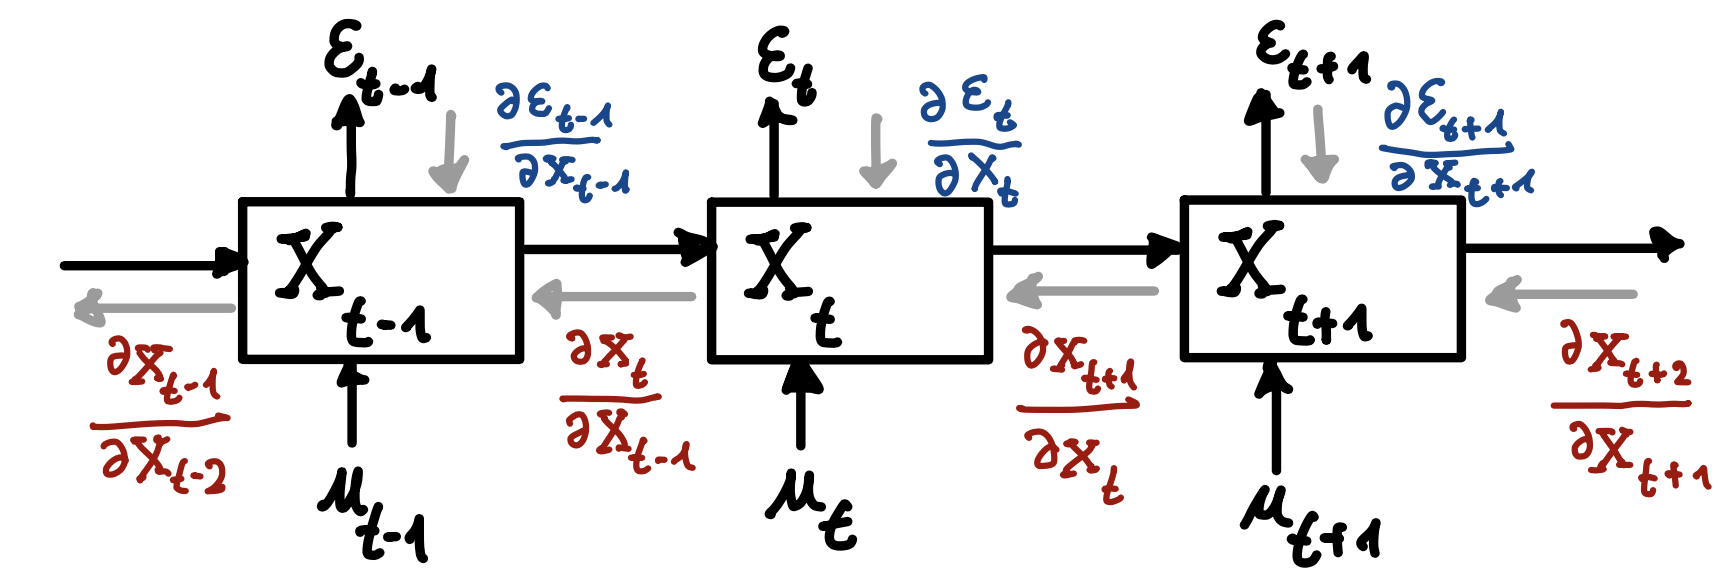
\includegraphics[width=0.95\linewidth]{figures/2_fig.png}\\[0.5em]
         Fig. 2: Unrolled RNN: Creating a copy of the model for each time step. \textcolor{myblue}{$\mathcal{E}_t$:}  error obtained at time step $t$ from the output |
          %\hspace{3em} 
          $\bullet$ \textcolor{myblue}{ \textit{total gradient over time}}
        \quad
        $\bullet$ \textcolor{myred}{ \textit{temporal error contribution}}


        \vspace{0.3em}
        \begin{align*}
          \textcolor{myblue}{\frac{\partial \mathcal{E}}{\partial \theta}} &=
          \sum_{t=1}^{T} \frac{\partial \mathcal{E}_t}{\partial \theta} \hspace{2em} \text{(3)} \\[0.5em]
          \frac{\partial \mathcal{E}_t}{\partial \theta} &=
          \sum_{k=1}^{t} 
          \left( {\frac{\partial \mathcal{E}_t}{\partial x_t}} 
          \textcolor{myred}{\frac{\partial x_t}{\partial x_k}}
          \frac{\partial^+ x_k}{\partial \theta} \right) \hspace{2em} \text{(4)} \\[0.5em]
          \textcolor{myred}{\frac{\partial x_t}{\partial x_k}} &=
          \prod_{i=k+1}^{t}
          \textcolor{orange}{W_{\text{rec}}}^\top \cdot \text{diag}\left(\sigma'(x_{i-1})\right) \hspace{2em} \text{(5)}
        \end{align*}
        
        \vspace{0.5em}
        where $\frac{\partial^+ x_k}{\partial \theta}$ denotes the “immediate” partial derivative (treating $x_{k-1}$ as constant).
        
        \vspace{0.5em}
        %$\bullet$ \textcolor{myblue}{ \textit{total gradient over time}}
        % \quad
        %$\bullet$ \textcolor{myred}{ \textit{temporal error contribution}}

      \end{block}





      \begin{block}{2. The Problem}

    \textbf{Mechanics of Exploding and Vanishing Gradients:} \\
    These issues occur in RNNs due to repeated multiplication of Jacobian matrices during backpropagation. If the spectral radius $\rho$ of the recurrent weight matrix $W_{\text{rec}}$ is less than 1, gradients vanish; if greater than 1, they explode. For non-linear activations with bounded derivatives (e.g., $\gamma=1$ for tanh), gradients vanish when the largest singular value $\lambda_1 < \gamma^{-1}$.

    \vspace{0.5em}
    \textbf{Dynamical Systems View:} \\
    An RNN's hidden state evolves like a dynamical system converging to attractors. As parameters change, the system may cross bifurcation points, causing drastic changes in state evolution. Crossing basin boundaries can result in gradient explosions. Inputs can shift the system into different attractor basins, intensifying this instability.
    \end{block}
    \end{column}

   %%%%%%%%%%%%%%%%%%%%%%%%%%%%%%%%%%%% Column 2 %%%%%%%%%%%%%%%%%%%%%%%%%%%%%%%%%%%%%%%%%%%%%%%%%%%%%%%%
\begin{column}{0.3\textwidth}
    \begin{block}{2. The Problem (cont.)}

    % \textbf{Mechanics of Exploding and Vanishing Gradients:} \\
    % These issues occur in RNNs due to repeated multiplication of Jacobian matrices during backpropagation. If the spectral radius $\rho$ of the recurrent weight matrix $W_{\text{rec}}$ is less than 1, gradients vanish; if greater than 1, they explode. For non-linear activations with bounded derivatives (e.g., $\gamma=1$ for tanh), gradients vanish when the largest singular value $\lambda_1 < \gamma^{-1}$.

    % \vspace{0.5em}
    % \textbf{Dynamical Systems View:} \\
    % An RNN's hidden state evolves like a dynamical system converging to attractors. As parameters change, the system may cross bifurcation points, causing drastic changes in state evolution. Crossing basin boundaries can result in gradient explosions. Inputs can shift the system into different attractor basins, intensifying this instability.

    \begin{center}
        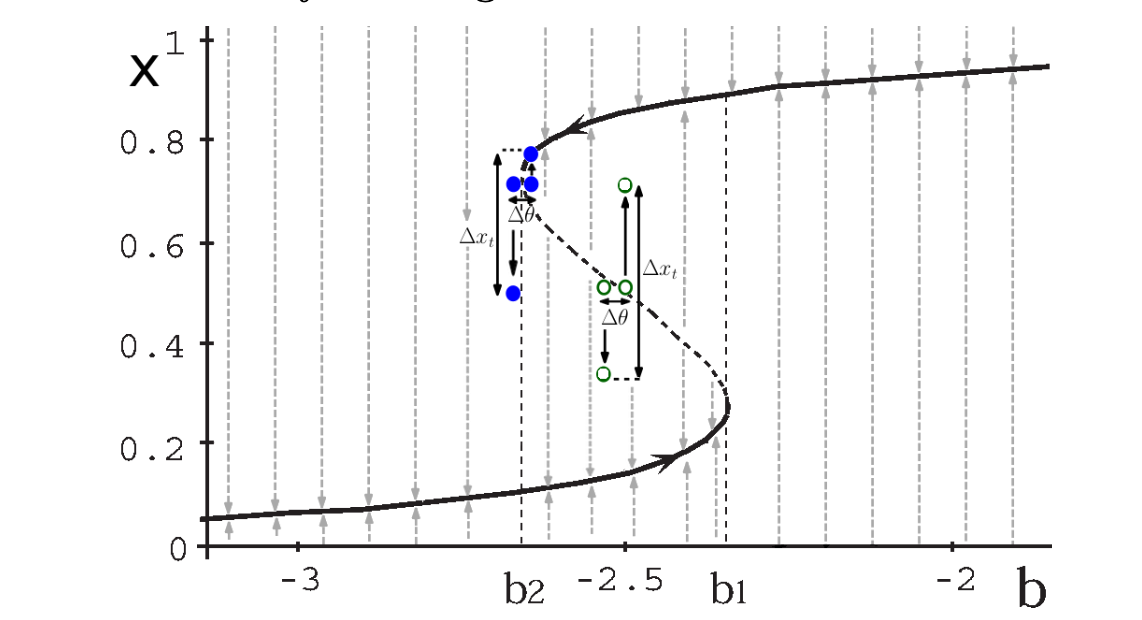
\includegraphics[width=0.9\linewidth]{figures/bifurcation.png} \\
        \small Bifurcation diagram showing attractor transitions
    \end{center}
    
    \begin{center}
        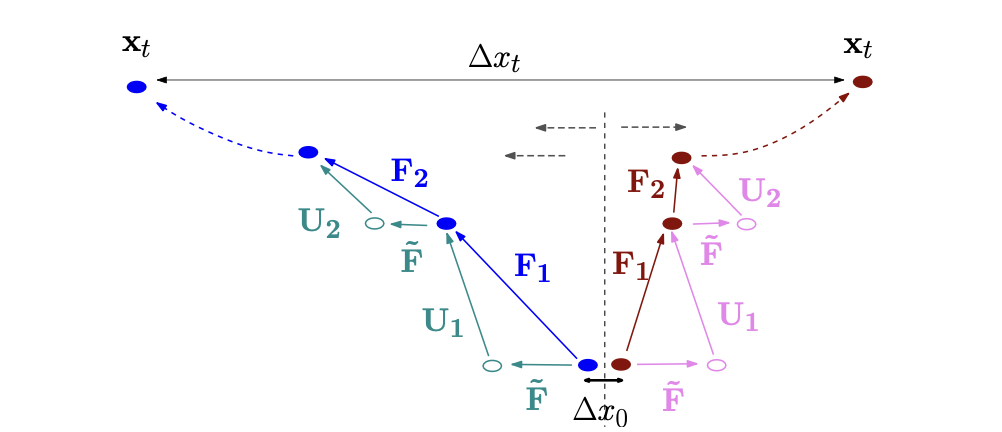
\includegraphics[width=0.9\linewidth]{figures/function_and_input.png} \\
        \small Gradient explosion due to basin crossing
    \end{center}

    \vspace{0.5em}
    \textbf{Geometric Interpretation:} \\
    Consider $x_t = w\sigma(x_{t-1}) + b$ with $x_0 = 0.5$. In the linear case ($b = 0$), gradients are $\frac{\partial x_t}{\partial w} = t w^{t-1} x_0$, showing exponential growth. Exploding gradients align with steep directions in the error surface, forming sharp walls that SGD struggles to traverse, disrupting convergence.

    \begin{center}
        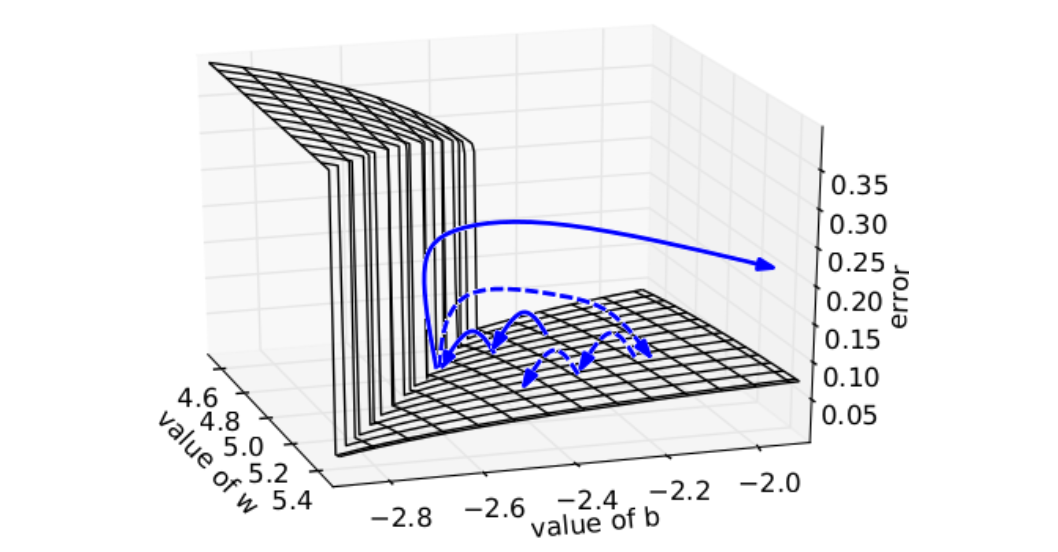
\includegraphics[width=0.9\linewidth]{figures/geometric.png} \\
        \small Steep error surface caused by exploding gradients
    \end{center}

    \end{block}



    \begin{block}{5. Relevance today \& SOTA techniques}
        %%% SUMMARY
        % \begin{table}[h!]
        % \centering
        % \begin{tabular}{|c|c|c|}
        % \hline
        % \textbf{Technique} & \textbf{Advantages} & \textbf{Disadvantages} \\ \hline
        % Gradient Clipping & Prevents exploding gradients & Requires tuning of threshold \\ \hline
        % Regularization & Mitigates vanishing gradients & May not fully prevent instability \\ \hline
        % Initialization Strategies & Improves convergence & Sensitive to parameter choice \\ \hline
        % \end{tabular}
        % \caption{Comparison of Techniques for Addressing Gradient Issues in RNNs}
        % \end{table}

 
            %%% reorganized bullet points below in more space-efficient way
        
            \begin{tabular}{@{}ll@{}}
                \textbf{Exploding gradients:} & \textbf{Clipping is still relevant!} \\
                \textbf{Vanishing gradients:} & 
                    \begin{minipage}[t]{0.8\textwidth} 
                        \textbf{Alternatives to regularization:}\\[0.3em]
                        \begin{tabular}{@{}lll@{}}
                        $\bullet$ Residual connections     & $\bullet$ Gating mechanisms       & $\bullet$ Attention mechanism \\
                        $\bullet$ Gradient checkpointing   & $\bullet$ Layer normalization     & $\bullet$ Positional encoding \\
                        \end{tabular}
                    \end{minipage} \\
                \end{tabular}
                
                \end{block}
    
\end{column}



    %%%%%%%%%%%%%%%%%%%%%%%%%%%%%%%%%%%% Column 3 %%%%%%%%%%%%%%%%%%%%%%%%%%%%%%%%%%%%%%%%%%%%%%%%%%%%%%%%
    \begin{column}{0.3\textwidth}
    % \begin{block}{3. Solution \& Experiments}
        \begin{block}{3. Solution }

        \textbf{Gradient Clipping}
        
        %\vspace{-2em}
    
        \begin{minipage}{0.54\textwidth}
        \begin{itemize}
          \item Pseudo-code: $\hat{g} \leftarrow \nabla E;\ \text{if } \|\hat{g}\|_2 \geq \tau \text{ then } \hat{g} \leftarrow \tau \cdot \frac{\hat{g}}{\|\hat{g}\|_2}$
          \item Gradient clipping introduces a hyperparameter: the threshold. A common heuristic sets this value based on the average gradient norm over early training steps.
          \item Compared to clipping individual gradient components by value, norm-based clipping preserves the direction of the gradient vector and is generally more robust in high-dimensional settings.
        \end{itemize}
        \end{minipage}
        \hfill
        \begin{minipage}{0.42\textwidth}
        \centering
        \vspace{1em} % pulls the image up
        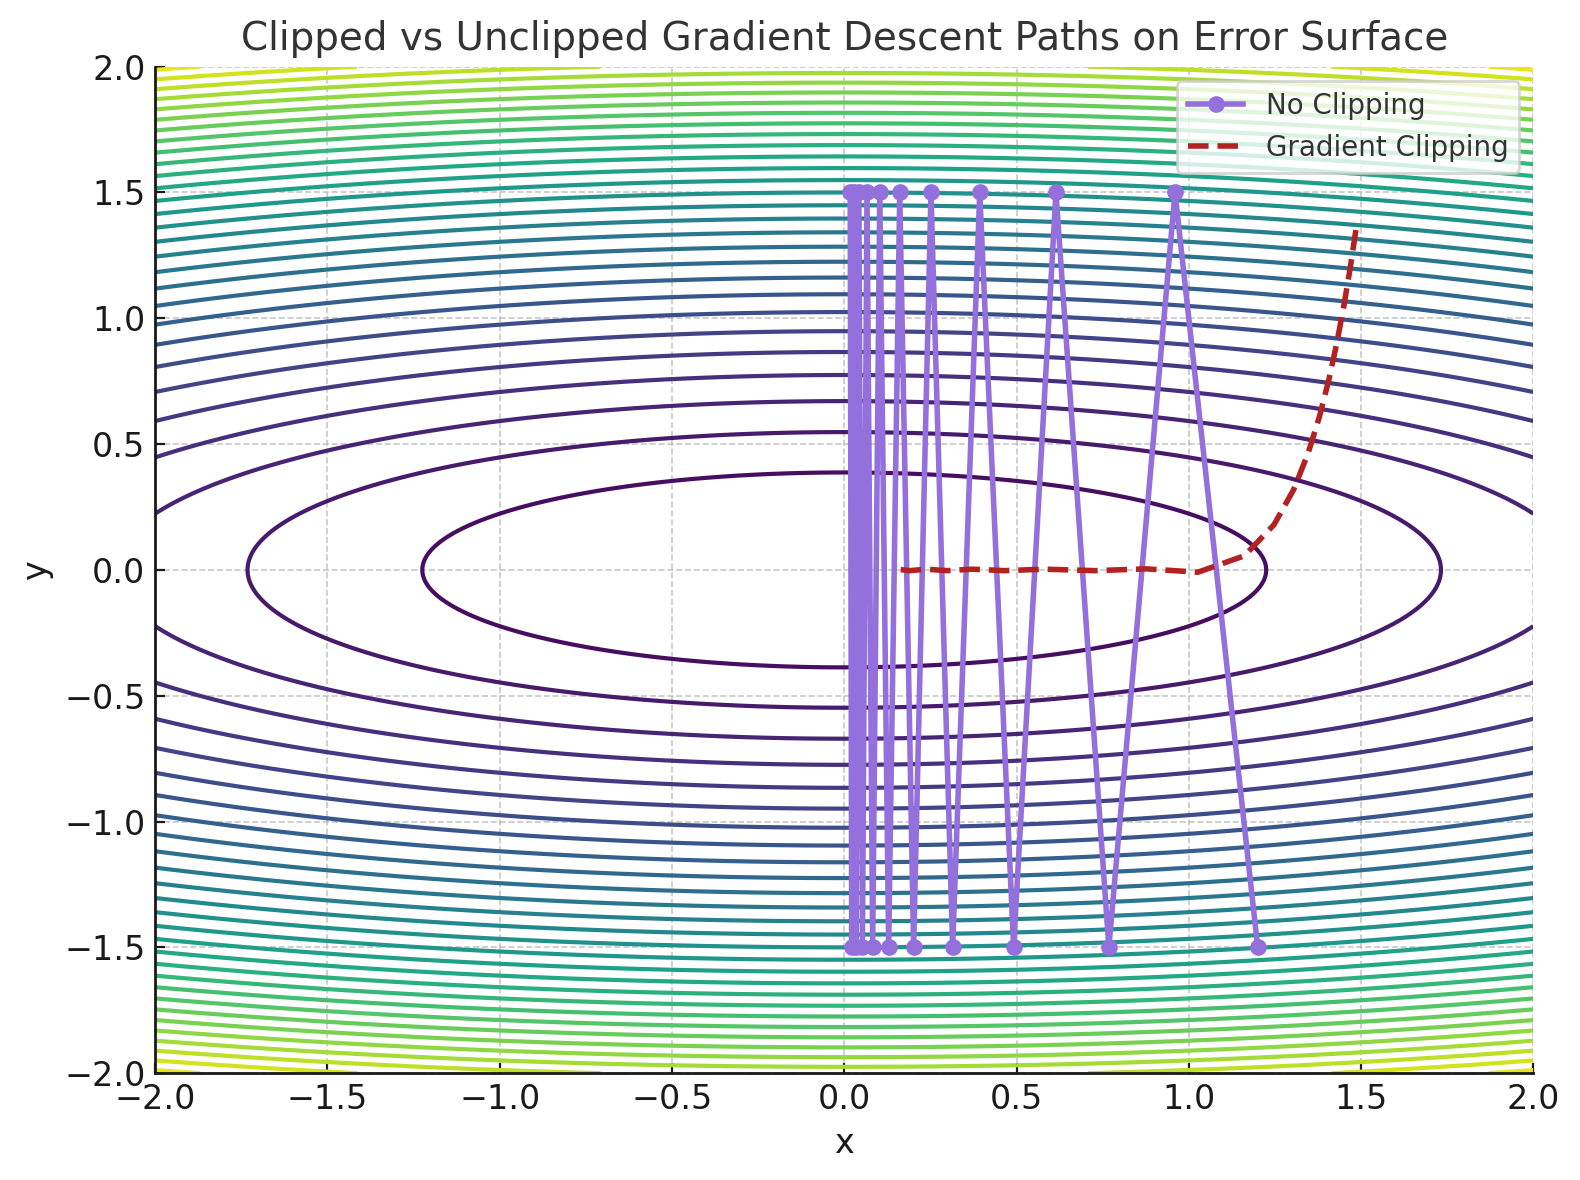
\includegraphics[width=\linewidth]{figures/gradient_clipping.png}
        % \vspace{-0.8em} % reduce space below
        \\[-0.3em]
        \end{minipage}

      \textbf{Vanishing Gradient Regularization}
      \begin{itemize}
        \item Regularizer: \[
            \Omega = \sum_k \Omega_k = \sum_k \left(  \frac{ \left\| \frac{\partial E}{\partial x_{k+1}} \cdot \frac{\partial x_{k+1}}{\partial x_k} \right\| }
            { \left\| \frac{\partial E}{\partial x_{k+1}} \right\| } - 1 
            \right)^2
            \]
            \[
            \textstyle
            \frac{\partial^+ \Omega}{\partial W_{\text{rec}}} = \sum_k 
            \frac{\partial^+}{\partial W_{\text{rec}}} \left(
            \left( 
            \frac{ \left\| \frac{\partial E}{\partial x_{k+1}} \cdot W_{\text{rec}}^\top \cdot \operatorname{diag}\left( \sigma'(x_k) \right) \right\|^2 }
            { \left\| \frac{\partial E}{\partial x_{k+1}} \right\|^2 } - 1 
            \right)^2
            \right)
            \]

        \item The regularization term only enforces norm preservation of the Jacobian matrix
                $\frac{\partial x_{k+1}}{\partial x_k}$ in the direction of the error signal 
                $\frac{\partial E}{\partial x_{k+1}}$, not in all directions.
        \item The soft constraint does not guarantee perfect norm preservation, so exploding gradients may still occur, particularly during early training or unstable updates. To mitigate this, we combine the regularizer with gradient clipping for more stable and effective learning.


      \end{itemize}
\end{block}
    \begin{block}{4. Experiments \& Results}

  %\textbf{Experiments and Results}
%   \begin{tikzpicture} 
% [mindmap,
%   grow cyclic,
%   every node/.style={concept,minimum size=4.2cm,inner sep=0pt,},
%   concept color=uniLightViolet2,
%   text width=7cm,
%   align=left,
%   level 1/.append style={level distance=10cm,font=\normalsize, minimum size=4.5cm, align=left,},
%   level 2/.append style={level distance=6cm, sibling angle=45, font=\small, minimum size=4cm, align=left,},
% ]
% \node [font=\normalsize, minimum size=5cm, align=flush center]{Two types\\of\\Problems}
%   child [grow=180,concept color=uniLightViolet2, align = left, minimum size=5cm] { node {{Pathological\\Problems}}
%     child [grow=60]{ node {Temporal\\Order\\ Problem}}
%     child [grow=100]{ node {Addition\\Problem}}
%     child [grow=145]{ node {Multiplication\\Problem}}
%     child [grow=190]{ node {3-bit\\Temporal\\ Problem}}
%     child [grow=245]{ node {Random\\Permutation\\Problem}}
%     child [grow=325] { node {Noiseless\\ Memorization\\ Problem}}
%   }
%   child [grow=0, concept color=uniLightViolet2,  minimum size=7cm, align=left] { node {Natural\\ Problems}
%     child [grow=60]{ node {Polyphonic\\Music\\Prediction}}
%     child [grow=135]{ node {Language\\Modeling\\(character level)}}
%   }
% ;
% \end{tikzpicture}
% Add vertical space after the mindmap
   \vspace{0.5cm}

  % Add the heading and 6-7 lines of text
  % \textbf{Experiments and Results To edit} \\
  \small{
  \begin{itemize}
    \item Datasets Utilized: Experiments leveraged synthetic pathological tasks (temporal order, addition, multiplication, 3-bit temporal order, random permutation, noiseless memorization) (Hochreiter and Schmidhuber (1997)), and natural datasets including polyphonic music prediction (Piano-midi.de, Nottingham, MuseData) and character-level language modeling (Penn Treebank), testing both short and long-term dependency learning.
    \item Temporal Order Problem Success: The temporal order problem showed that gradient clipping (MSGD-C) and regularization (MSGD-CR) improved success rates over standard mini-batch SGD (MSGD), especially for longer sequences.
    \item Impact of Initialization: Three initializations (sigmoid, basic tanh, smart tanh) were compared, with "smart tanh" (sparse W\_rec, spectral radius 0.95) performing best, highlighting initialization's role in RNN training.
    \item Clipping Importance: Gradient clipping was critical for tasks needing long memory traces, as longer sequences correlated with larger spectral radii, increasing the likelihood of exploding gradients.
    \item Generalization Across Lengths: A single model trained with MSGD-CR handled sequences from 50 to 200 steps with 100\% success and generalized to unseen lengths up to 5000 steps, suggesting robust long-term memory. 
    \item Other Pathological Tasks: MSGD-CR solved multiple tasks (addition, multiplication, 3-bit temporal order, random permutation, noiseless memorization) with near-perfect success for sequences up to 200 steps, outperforming prior work. 
    \item Natural Problems Tested: The solutions were applied to real-world tasks: polyphonic music prediction (Piano-midi.de, Nottingham, MuseData) and character-level language modeling (Penn Treebank). 
    \item Clipping as Optimization: Clipping improved both training and test errors in natural tasks, indicating it addresses optimization issues rather than acting as a regularizer. 
    \item Regularization Challenges: Fixed regularization weights harmed short-term correlation learning in natural tasks; a decreasing schedule (halving) was needed, suggesting a trade-off between short- and long-term dependencies. 
    \item SOTA Results: For Penn Treebank, MSGD-CR matched RNN SOTA results; for music prediction, it achieved RNN state-of-the-art, though RNN-NADE performed better overall, validating the clipping strategy. 
  \end{itemize}}  % end small
  % Add vertical space before the image
  \vspace{0.5cm}
\begin{center}
  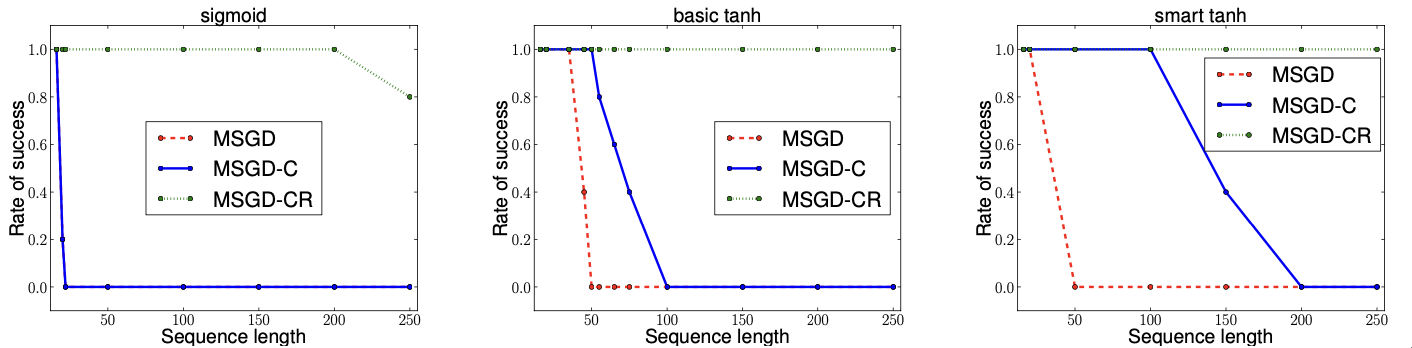
\includegraphics[width=0.9\textwidth]{figures/results.png}
  %\vspace{0.2cm}
  \captionof{\\Figure 7: Rate of success for solving the temporal order problem versus sequence length for different initializations (from left to right: sigmoid, basic tanh and smart tanh)}
\end{center}
 \vspace{0.5cm}


% if using 3 images separately
% \begin{figure}[h]
%   \centering
%   \begin{minipage}{0.3\textwidth}
%     \centering
%     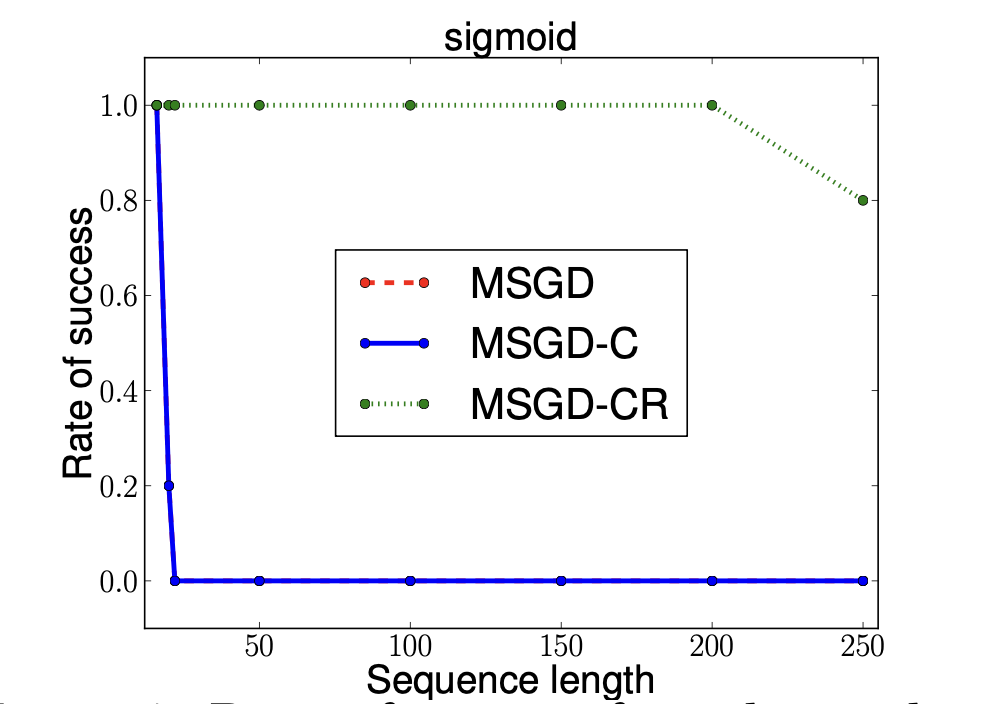
\includegraphics[width=\textwidth]{figures/sigmoid.png}
%     \caption{sigmoid.png}
%   \end{minipage}\hfill
%   \begin{minipage}{0.3\textwidth}
%     \centering
%     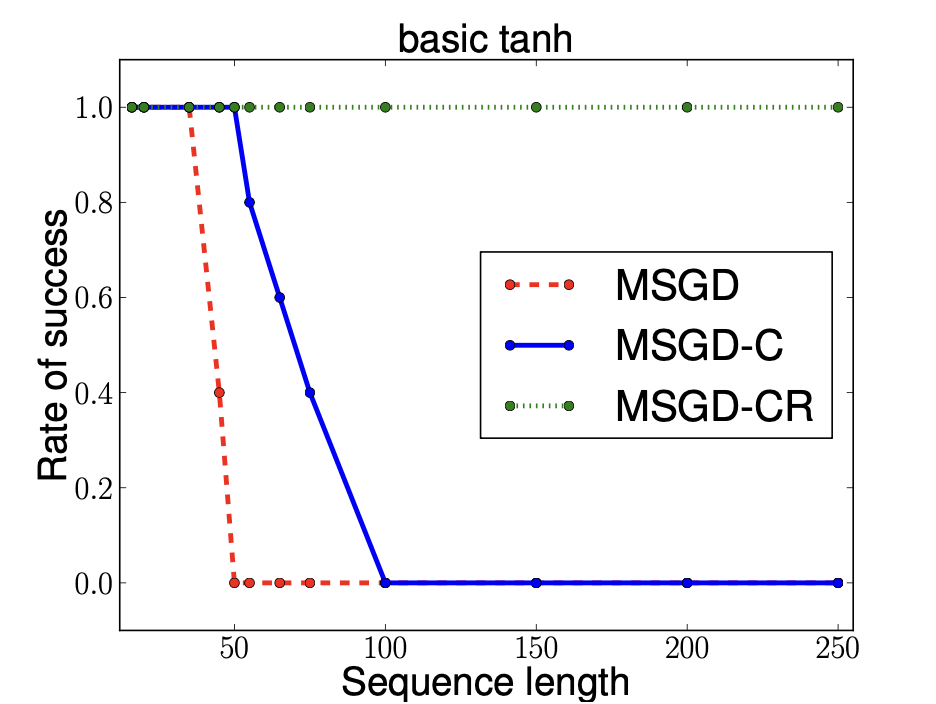
\includegraphics[width=\textwidth]{figures/basic_tanh.png}
%     \caption{basic_tanh.png}
%   \end{minipage}\hfill
%   \begin{minipage}{0.3\textwidth}
%     \centering
%     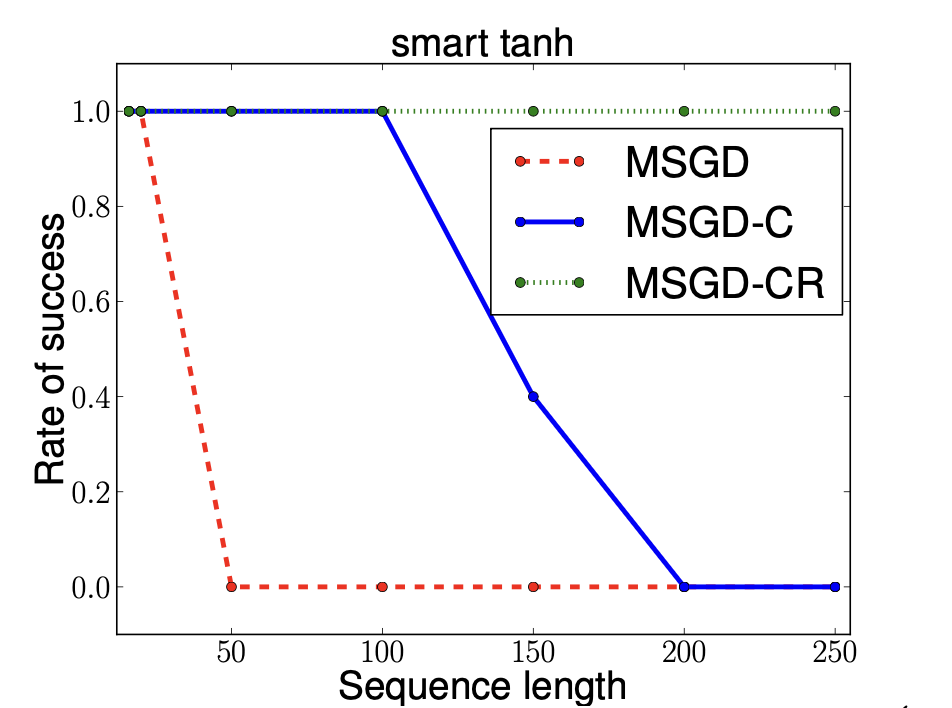
\includegraphics[width=\textwidth]{figures/smart_tanh.png}
%     \caption{smart_tanh.png}
%   \end{minipage}
% \end{figure}

    \end{block}

    %\vspace{1em}
  
    % \begin{block}{5. Relevance today \& SOTA techniques}
    %     %%% SUMMARY
    %     % \begin{table}[h!]
    %     % \centering
    %     % \begin{tabular}{|c|c|c|}
    %     % \hline
    %     % \textbf{Technique} & \textbf{Advantages} & \textbf{Disadvantages} \\ \hline
    %     % Gradient Clipping & Prevents exploding gradients & Requires tuning of threshold \\ \hline
    %     % Regularization & Mitigates vanishing gradients & May not fully prevent instability \\ \hline
    %     % Initialization Strategies & Improves convergence & Sensitive to parameter choice \\ \hline
    %     % \end{tabular}
    %     % \caption{Comparison of Techniques for Addressing Gradient Issues in RNNs}
    %     % \end{table}

 
    %         %%% reorganized bullet points below in more space-efficient way
        
    %         \begin{tabular}{@{}ll@{}}
    %             \textbf{Exploding gradients:} & \textbf{Clipping is still relevant!} \\
    %             \textbf{Vanishing gradients:} & 
    %                 \begin{minipage}[t]{0.8\textwidth} 
    %                     \textbf{Alternatives to regularization:}\\[0.3em]
    %                     \begin{tabular}{@{}lll@{}}
    %                     $\bullet$ Residual connections     & $\bullet$ Gating mechanisms       & $\bullet$ Attention mechanism \\
    %                     $\bullet$ Gradient checkpointing   & $\bullet$ Layer normalization     & $\bullet$ Positional encoding \\
    %                     \end{tabular}
    %                 \end{minipage} \\
    %             \end{tabular}
                
    
                

    %   \begin{itemize}
    %     \item Clipping still relevant!
    %     \item Instead of regularization:
    %     \begin{itemize}
    %       \item residual connections
    %       \item gradient checkpointing
    %       \item gating mechanisms
    %       \item layer normalization
    %       \item attention mechanism
    %       \item positional encoding
    %     \end{itemize}
    %   \end{itemize}
    %\end{block}
    \hspace{2em}
  \end{column}
  
  \end{columns}
\end{frame}

\end{document}
